% The seven quadratic extensions of Q_2, sorted by ramification (generated by a script).
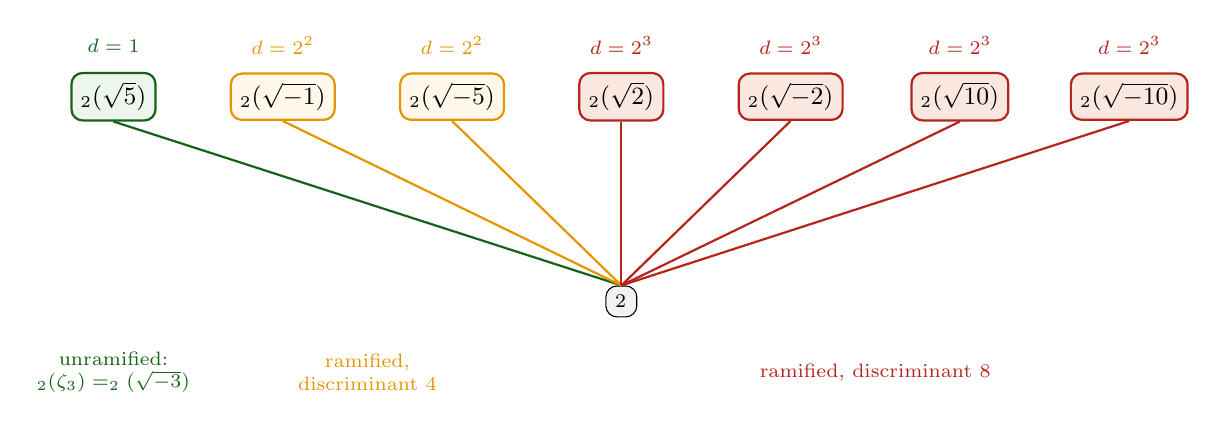
\begin{tikzpicture}[x=2.15cm,y=1cm]
\node[draw,rounded corners,fill=black!5] (Q) at (3,0) {$\Q_2$};
\node[draw=ForestGreen!70!black,thick,rounded corners,fill=ForestGreen!8,font=\small] (E0) at (0,2.6) {$\Q_2(\sqrt5)$};
\draw[ForestGreen!70!black,thick] (Q.north)--(E0.south);
\node[font=\scriptsize,ForestGreen!70!black] at (0,3.25) {$d=1$};
\node[draw=Orange!90!black,thick,rounded corners,fill=Orange!8,font=\small] (E1) at (1,2.6) {$\Q_2(\sqrt{-1})$};
\draw[Orange!90!black,thick] (Q.north)--(E1.south);
\node[font=\scriptsize,Orange!90!black] at (1,3.25) {$d=2^2$};
\node[draw=Orange!90!black,thick,rounded corners,fill=Orange!8,font=\small] (E2) at (2,2.6) {$\Q_2(\sqrt{-5})$};
\draw[Orange!90!black,thick] (Q.north)--(E2.south);
\node[font=\scriptsize,Orange!90!black] at (2,3.25) {$d=2^2$};
\node[draw=BrickRed,thick,rounded corners,fill=BrickRed!8,font=\small] (E3) at (3,2.6) {$\Q_2(\sqrt2)$};
\draw[BrickRed,thick] (Q.north)--(E3.south);
\node[font=\scriptsize,BrickRed] at (3,3.25) {$d=2^3$};
\node[draw=BrickRed,thick,rounded corners,fill=BrickRed!8,font=\small] (E4) at (4,2.6) {$\Q_2(\sqrt{-2})$};
\draw[BrickRed,thick] (Q.north)--(E4.south);
\node[font=\scriptsize,BrickRed] at (4,3.25) {$d=2^3$};
\node[draw=BrickRed,thick,rounded corners,fill=BrickRed!8,font=\small] (E5) at (5,2.6) {$\Q_2(\sqrt{10})$};
\draw[BrickRed,thick] (Q.north)--(E5.south);
\node[font=\scriptsize,BrickRed] at (5,3.25) {$d=2^3$};
\node[draw=BrickRed,thick,rounded corners,fill=BrickRed!8,font=\small] (E6) at (6,2.6) {$\Q_2(\sqrt{-10})$};
\draw[BrickRed,thick] (Q.north)--(E6.south);
\node[font=\scriptsize,BrickRed] at (6,3.25) {$d=2^3$};
\node[font=\scriptsize,align=center,ForestGreen!70!black] at (0,-0.9) {unramified:\\ $\Q_2(\zeta_3)=\Q_2(\sqrt{-3})$};
\node[font=\scriptsize,align=center,Orange!90!black] at (1.5,-0.9) {ramified,\\ discriminant $4$};
\node[font=\scriptsize,align=center,BrickRed] at (4.5,-0.9) {ramified, discriminant $8$};
\end{tikzpicture}
